\documentclass[12pt,a4paper]{article}
\usepackage[T1]{fontenc}
\usepackage[utf8]{inputenc}
\usepackage[italian]{babel}
\usepackage{amsmath,amsfonts}
\usepackage{amssymb}
\usepackage{mathtools}
\usepackage{multicol}
\usepackage{array}
\usepackage{pdflscape}
\usepackage[dvipsnames]{xcolor}
\usepackage{colortbl}
\usepackage{graphicx}
\usepackage{wrapfig}	% per didascalie avvolte nel testo
\usepackage{booktabs}
\usepackage{multirow}
\usepackage{parskip}	% pacchetto per la non indentazione del paragrafo
\usepackage{enumitem}	% per elenchi con label
\usepackage{subcaption} 	% più performante rispetto subfigure
\usepackage{geometry}	% cambiare la geometria del decumento
\usepackage{tabularx}	% per stabilire autonomamente la larghezza delle tabelle
\usepackage{rotating}   % per ruotare le scritte all'interno delle tabelle
\usepackage{sidecap}	% per le didascalie laterali
\usepackage{longtable}	% per fare tabelle più lunghe di una pagina
\usepackage{eurosym}    % per mettere il simbolo dell'euro
\usepackage{adjustbox}  % per rendere le tabelle più piccole
\usepackage{verbatim}	% per usare l'ambiente comment
\usepackage{pdfpages}	% per includere pdf

% licenza
\usepackage{xmpincl}	% permette di includere licenze in formato XMP
%\includexmp{files/CC_Attribution-NonCommercial-ShareAlike_4.0_International}	% file della licenza

% bibliografia
\usepackage[autostyle,italian=guillemets]{csquotes}	% per citare con le virgolette giuste
\usepackage[bibstyle=authoryear,citestyle=authoryear-ibid,backend=biber]{biblatex}	% per la bib
\addbibresource{99-bibliografia.bib}
%\defbibheading{cartaceo}{\section*{Bibliografia cartacea}}
%\defbibheading{web}{\section*{Sitografia}}

% per scrivere bene le unità di misura
\usepackage{siunitx}
\sisetup{
	output-decimal-marker	=	{.},
	list-final-separator	=	{ e },
	list-pair-separator		=	{ e },
	range-phrase			=	{ a },
	per-mode				=	symbol,
    sticky-per 				=	true,
    detect-all				=	true,
}
\DeclareSIUnit\anni{anni}
\DeclareSIUnit\anno{anno}
\DeclareSIUnit\minuti{minuti}
\DeclareSIUnit\minuto{minuto}
\DeclareSIUnit\ore{ore}
\DeclareSIUnit\ora{ora}
\DeclareSIUnit\none{-}
\DeclareSIUnit\e{\euro}

% per personalizzare le caption
\usepackage{caption}
\captionsetup{
	labelformat=simple, % simple senza parentesi, parens con le parentesi
	font={it},
	labelfont=bf,
	justification=centerlast
}

% pacchetto per personalizzare le testatine
\begin{comment}
\usepackage{fancyhdr}
\pagestyle{fancy}
\renewcommand{\chaptermark}[1]{\markboth{#1}{}}
\renewcommand{\sectionmark}[1]{\markright{\thesection\ #1}}
\fancyhf{}
\fancyhead[RO]{\bfseries\rightmark}
\fancyhead[LE]{\bfseries\leftmark}
\fancyfoot[C]{\thepage}
\renewcommand{\headrulewidth}{0.5pt}
\renewcommand{\footrulewidth}{0pt}
\setlength{\headheight}{14pt}
\end{comment}

% serie di pacchetti per la stesura con Latex di grafici e disegni
\usepackage{tikz}
\usepackage{pgfplots}	% pacchetto per grafici
\pgfplotsset{compat=newest}	% ultima versione
\SendSettingsToPgf
\usepgfplotslibrary{fillbetween}	% per riempire di colore i grafici
\usepgfplotslibrary{dateplot}	% per usare date come numeri
\usepgfplotslibrary{external}	% per creare pdf esterni dei grafici
%\tikzexternalize

% per riferimenti
\usepackage{hyperref}
\hypersetup{
	colorlinks	=	true,	% attiva il colore per i link, altrimenti sono inscatolati
	%linkcolor	=	black,	% il colore dei link è nero
	pdftitle	=	Tesi: Dinamiche vegetazionali nel fiume Tagliamento,
	pdfauthor	=	 Castellani Robin,
	%hidelinks,
}



\begin{document}
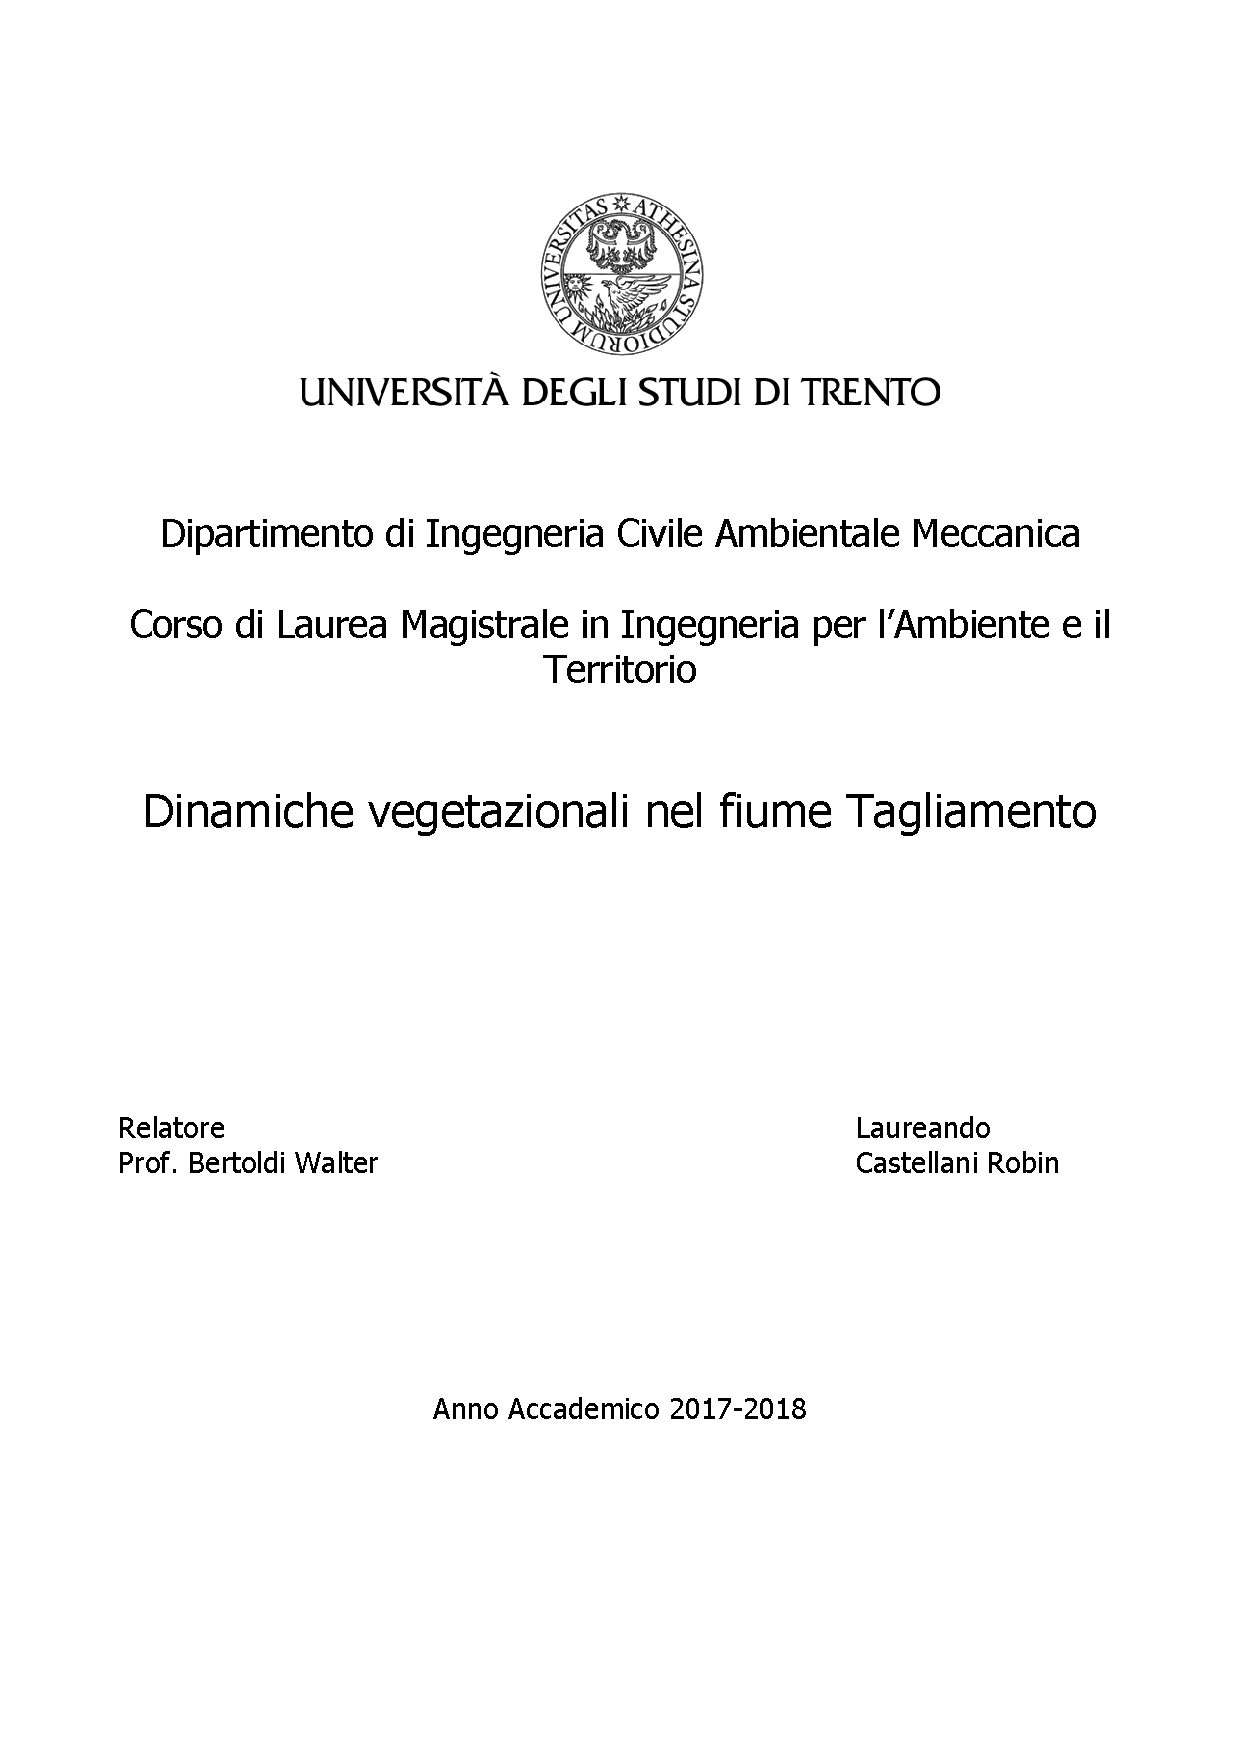
\includepdf[pages=-]{files/frontespizio.pdf}

\pagenumbering{roman}
%----------------------------------------------------------
\begin{abstract}
La presente tesi mira a studiare come cambia la vegetazione nel fiume braided Tagliamento in risposta all'idrologia. 
L'obiettivo principale è quello di ricercare una relazione tra i livelli del pelo libero registrati da alcuni idrometri e la vegetazione erosa, tra i livelli e la quantità di legname che si ritrova in alveo.

Si analizzano immagini satellitari e ortofoto al fine di distinguere la parte vegetata dell'alveo e il legname presente.
Con i dati di piovosità media mensile e di temperatura media mensile si cercano correlazioni con l'espansione della vegetazione che si osserva negli anni.
Dalla quantificazione dell'erosione della vegetazione dovuta alle piene, della quantità di legno in alveo e di un tasso di crescita della vegetazione si tenta di costruire un bilancio di materia vegetale a scala di evento di piena.
Inoltre si trovano valori soglia per l'erosione della vegetazione.
\end{abstract}
%----------------------------------------------------------

\clearpage

\pagenumbering{arabic}
Il grafico~\ref{graph:livelli-orto-sat} mostra i livelli idrometrici registrati presso l'idrometro di Villuzza, corrispondente al ponte di Pinzano; sono inoltre mostrati con delle linee le date di cui si dispongono immagini satellitari (ASTER, Pleiades, Sentinel2, Google~Earth) e ortofoto.
La tabella~\ref{tab:date-orto-sat} mostra le date e la risoluzione delle immagini utilizzate nell'analisi.

\begin{figure}[ht]
	\centering
	\begin{tikzpicture}
	%\begin{groupplot}
	\begin{axis}[
		%name = orto-sat,
		axis y line* = right,
		axis x line* = top,
		%height = .3\textwidth,
		width = \textwidth,
		date coordinates in = x,
		%symbolic y coords = {ASTER,PLEIADES,SENTINEL2,G-EARTH},
		xticklabel = {\year-\month-\day},
		xtick = data,
		ytick = data,
		xticklabel style = {
			rotate = 90,
			anchor = near xticklabel
		},
		enlarge x limits = 0.05,
		enlarge y limits = 0.01,
		ylabel = {Fonte},
		ymax = 3.6,
		ymin = -0.1,
		grid = none,
		only marks,
		]
		\addplot table [x=data, y=numero] {graphics/data/data-orto-sat.txt};
	\end{axis}
	%
	\begin{axis}[
		%name = stages,
		%at = {($(orto-sat.south)-(0,2cm)$)},
		%anchor = north,
		axis y line* = left,
		width = \textwidth,
		date coordinates in = x,
		xticklabel = {\year-\month-\day},
		xticklabel style = {
			rotate = 45,
			anchor = near xticklabel
		},
		enlarge x limits = 0.05,
		enlarge y limits = 0.01,
		ymax = 3.6,
		ymin = -0.1,
		ylabel = {Livello idrometrico},
		grid = major,
		no markers,
		]
		\addplot table [x=data, y=media-gg] {graphics/data/Dati_Villuzza.csv};
	\end{axis}
\end{tikzpicture}
	\caption[livelli idrometrici e foto aeree - satellitari]{livello idrometrico (in blu) presso l'idrometro di Villuzza. 
	Le linee indicano le immagini satellitari e le ortofoto considerate (ASTER in magenta, Pleiades in verde~acqua, Sentinel2 in azzurro, G-Earth in verde).}
	\label{graph:livelli-orto-sat}
\end{figure}




\begin{table}[ht]
	\centering
	\begin{tabular}{c c S[table-format=2.1]}
		\toprule
		Data		&	Fonte		&	\multicolumn{1}{c}{Risoluzione \si{[\m]}}	\\
		\midrule	
		2000-09-17	&	ASTER	&	15	\\
		2001-06-07	&	ASTER	&	15	\\
		2001-12-09	&	ASTER	&	15	\\
		2002-05-18	&	ASTER	&	15	\\
		2002-06-12	&	ASTER	&	15	\\
		2003-06-22	&	ASTER	&	15	\\
		2003-11-29	&	ASTER	&	15	\\
		2004-10-14	&	ASTER	&	15	\\
		2005-08-30	&	ASTER	&	15	\\
		2006-07-16	&	ASTER	&	15	\\
		2007-09-21	&	ASTER	&	15	\\
		2008-07-05	&	ASTER	&	15	\\
		2009-07-08	&	ASTER	&	15	\\
		2010-09-29	&	ASTER	&	15	\\
		2012-08-01	&	ASTER	&	15	\\
		2013-09-05	&	ASTER	&	15	\\
		2014-09-08	&	ASTER	&	15	\\
		2014-10-31	&	Pleiades	&	0.5	\\
		2015-09-11	&	ASTER	&	15	\\
		2015-09-29	&	Sentinel2	&	10	\\
		2016-09-13	&	Sentinel2	&	10	\\
		2017-04-21	&	Sentinel2	&	10	\\
		2017-07-07	&	G-Earth	&	0.45	\\
		\bottomrule
	\end{tabular}
	\caption{data e risoluzione delle immagini satellitari e delle ortofoto utilizzate.}
	\label{tab:date-orto-sat}
\end{table}



\begin{figure}[ht]
	\centering
	\begin{tikzpicture}
	\begin{axis}[
		width = \textwidth,
		height = 0.5\textwidth,
		date coordinates in = x,
		date ZERO = 2000-01-01,
		xticklabel = {\year},
		xticklabel style = {
			rotate = 80,
			anchor = near xticklabel
		},
		axis y line* = right,
		ymax = 70,
		%ymin = 0,
		ylabel = {Percentuale di vegetazione},
		grid = none,
		]
		\addplot+
        	[red, mark=+, ultra thick]
        	table [x=data, y=veg] {graphics/data/Class_sat_veg-H2O-ghiaia.txt};
	\end{axis}
	
	\begin{axis}[
		width = \textwidth,
		height = 0.5\textwidth,
		date coordinates in = x,
		date ZERO = 2000-01-01,
		xticklabel = {\year},
		xticklabel style = {
			rotate = 80,
			anchor = near xticklabel
		},
		axis y line* = left,
		axis x line = none,
		enlarge x limits = 0.05,
		enlarge y limits = 0.01,
		ymax = 3.7,
		ymin = 2,
		ylabel = {Livello idrometrico},
		grid = none,
		]
		\addplot+
        	[blue, no markers, ultra thin]
        	table [x=data, y=media-gg] {graphics/data/Dati_Villuzza.csv};
	\end{axis}
\end{tikzpicture}

	\caption[andamento dell'areale della vegetazione nelle isole  e nella floodplain]{andamento dell'areale della vegetazione nelle isole e nella floodplain. I dati provengono dalla classificazione delle immagini satellitari (ASTER, Pleiades e Sentinel2).}
	\label{graph:class-sat-veg}
\end{figure}


\clearpage



\printbibliography

\end{document}
